\section{mo\-Move\-Select$<$ M $>$ Class Template Reference}
\label{classmo_move_select}\index{moMoveSelect@{moMoveSelect}}
Class that describes a move selector ({\bf mo\-Move}{\rm (p.\,\pageref{classmo_move})}).  


{\tt \#include $<$mo\-Move\-Select.h$>$}

Inheritance diagram for mo\-Move\-Select$<$ M $>$::\begin{figure}[H]
\begin{center}
\leavevmode
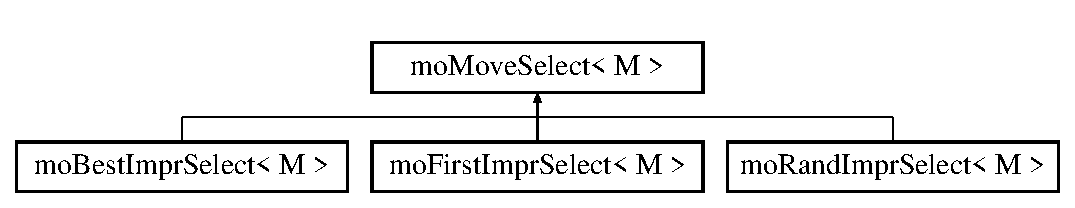
\includegraphics[height=2.82828cm]{classmo_move_select}
\end{center}
\end{figure}
\subsection*{Public Types}
\begin{CompactItemize}
\item 
typedef M::EOType::Fitness {\bf Fitness}\label{classmo_move_select_w0}

\begin{CompactList}\small\item\em Alias for the fitness. \item\end{CompactList}\end{CompactItemize}
\subsection*{Public Member Functions}
\begin{CompactItemize}
\item 
virtual void {\bf init} (const {\bf Fitness} \&\_\-fitness)=0
\begin{CompactList}\small\item\em Procedure which initialises all that the move selector needs including the initial fitness. \item\end{CompactList}\item 
virtual bool {\bf update} (const M \&\_\-move, const {\bf Fitness} \&\_\-fitness)=0
\begin{CompactList}\small\item\em Function which updates the best solutions. \item\end{CompactList}\end{CompactItemize}


\subsection{Detailed Description}
\subsubsection*{template$<$class M$>$ class mo\-Move\-Select$<$ M $>$}

Class that describes a move selector ({\bf mo\-Move}{\rm (p.\,\pageref{classmo_move})}). 

It iteratively considers some moves ({\bf mo\-Move}{\rm (p.\,\pageref{classmo_move})}) and their associated fitnesses. The best move is so regularly updated. At any time, it could be accessed. 



Definition at line 50 of file mo\-Move\-Select.h.

\subsection{Member Function Documentation}
\index{moMoveSelect@{mo\-Move\-Select}!init@{init}}
\index{init@{init}!moMoveSelect@{mo\-Move\-Select}}
\subsubsection{\setlength{\rightskip}{0pt plus 5cm}template$<$class M$>$ virtual void {\bf mo\-Move\-Select}$<$ M $>$::init (const {\bf Fitness} \& {\em \_\-fitness})\hspace{0.3cm}{\tt  [pure virtual]}}\label{classmo_move_select_a0}


Procedure which initialises all that the move selector needs including the initial fitness. 

In order to know the fitness of the solution, for which the neighborhood will be soon explored

\begin{Desc}
\item[Parameters:]
\begin{description}
\item[{\em \_\-fitness}]the current fitness. \end{description}
\end{Desc}


Implemented in {\bf mo\-Best\-Impr\-Select$<$ M $>$} {\rm (p.\,\pageref{classmo_best_impr_select_a0})}, {\bf mo\-First\-Impr\-Select$<$ M $>$} {\rm (p.\,\pageref{classmo_first_impr_select_a0})}, and {\bf mo\-Rand\-Impr\-Select$<$ M $>$} {\rm (p.\,\pageref{classmo_rand_impr_select_a0})}.\index{moMoveSelect@{mo\-Move\-Select}!update@{update}}
\index{update@{update}!moMoveSelect@{mo\-Move\-Select}}
\subsubsection{\setlength{\rightskip}{0pt plus 5cm}template$<$class M$>$ virtual bool {\bf mo\-Move\-Select}$<$ M $>$::update (const M \& {\em \_\-move}, const {\bf Fitness} \& {\em \_\-fitness})\hspace{0.3cm}{\tt  [pure virtual]}}\label{classmo_move_select_a1}


Function which updates the best solutions. 

\begin{Desc}
\item[Parameters:]
\begin{description}
\item[{\em \_\-move}]a new move. \item[{\em \_\-fitness}]a fitness linked to the new move. \end{description}
\end{Desc}
\begin{Desc}
\item[Returns:]a boolean that expresses the need to resume the exploration. \end{Desc}


Implemented in {\bf mo\-Best\-Impr\-Select$<$ M $>$} {\rm (p.\,\pageref{classmo_best_impr_select_a1})}, {\bf mo\-First\-Impr\-Select$<$ M $>$} {\rm (p.\,\pageref{classmo_first_impr_select_a1})}, and {\bf mo\-Rand\-Impr\-Select$<$ M $>$} {\rm (p.\,\pageref{classmo_rand_impr_select_a1})}.

The documentation for this class was generated from the following file:\begin{CompactItemize}
\item 
mo\-Move\-Select.h\end{CompactItemize}
